\documentclass{tufte-book}
\usepackage{tikz}
\usepackage{amsmath,amsthm,amssymb}
\usepackage{esint}
\usepackage{geometry}
\usepackage{setspace}
\usepackage{graphicx}
\usepackage{calc}
\usepackage{scalerel}
\usepackage{eso-pic}
\graphicspath{ {../images/} }

% custom script-r
\renewcommand{\b}{\mathbf}
\newcommand{\h}[1]{\mathbf{\hat{#1}}}
\def\r{{\mbox{$\resizebox{.09in}{.08in}{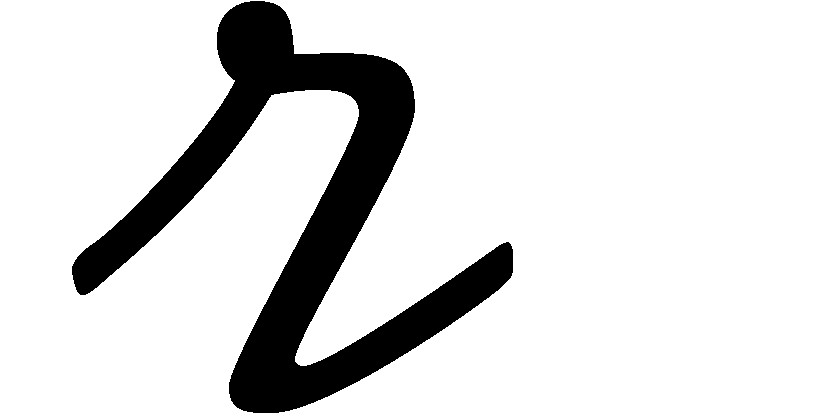
\includegraphics[trim= 1em 0 14em 0,clip]{ScriptR}}$}}}
\def\br{{\mbox{$\resizebox{.09in}{.08in}{
\includegraphics[trim= 1em 0 14em 0,clip]{BoldR}}$}}}


% title
\setlength{\parindent}{0pt}
\title{Electromagnetism}
\author{Richard Robinson}
\begin{document}
\maketitle
\setlength{\parindent}{0pt}

%-------------------------------------------

\chapter{Electrostatics}

\section{Electric Forces}
\textsc{In Electrodynamics}, there is typically a \emph{source point} $\b r '$ where a charge is located and a \emph{field point} $\b r$ where a field is calculated at. The \emph{seperation vector} is defined as
\begin{equation}
  \br \equiv \b r - \b r ' \qquad \hat\br = \br/\r
\end{equation}
The force acting on a charge is given by \emph{Coulomb's Law}, \begin{equation}
  \b F = k \sum \frac{q_1q_2}{\r^2} \hat\br = \iiint d \b F
\end{equation}
%
\begin{marginfigure}
  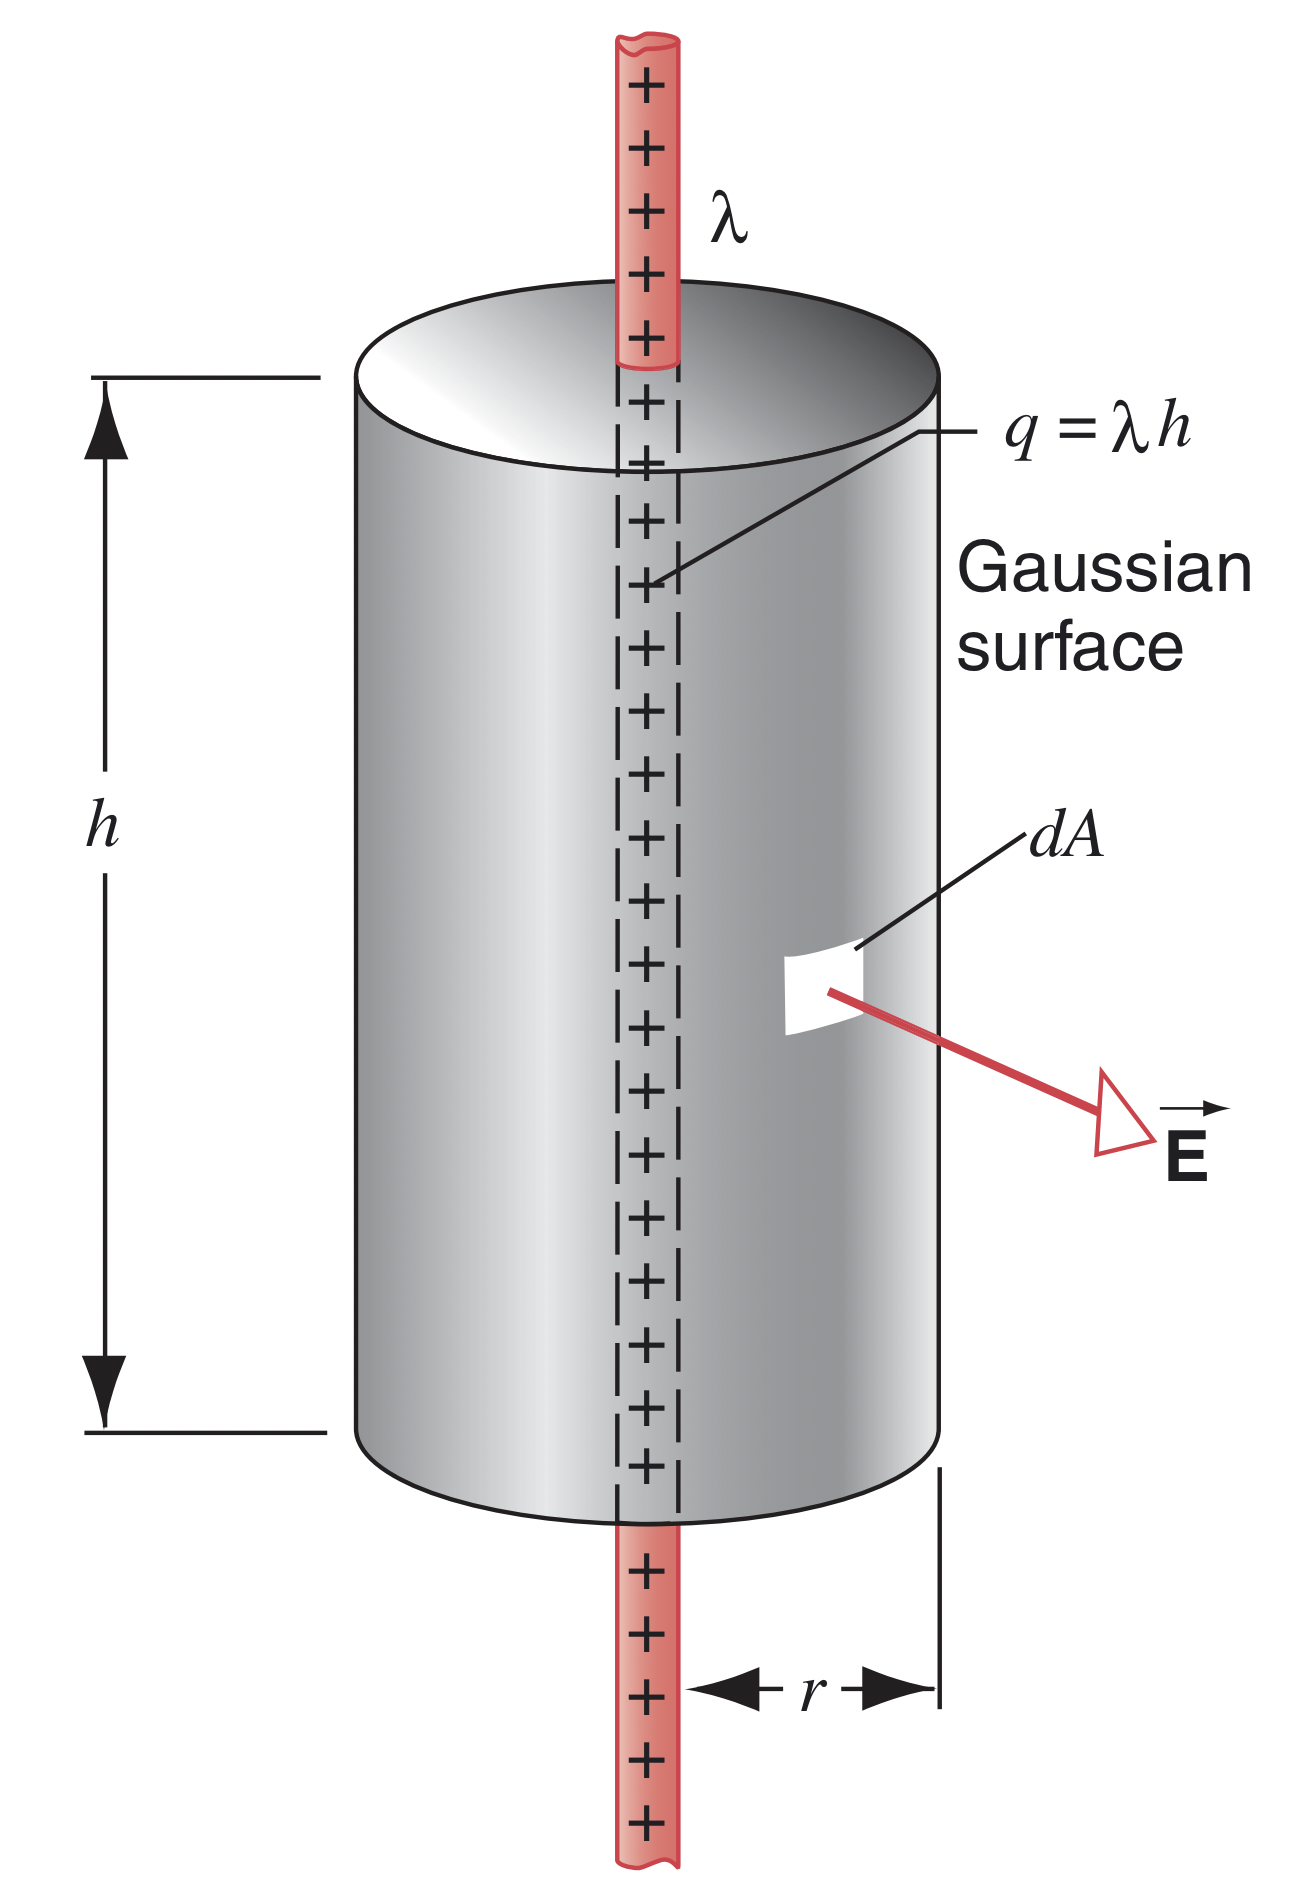
\includegraphics[scale=0.15]{field}
  \caption{A Gaussian surface as a cylinder.}
\end{marginfigure}
%
The \emph{electric field} exerted on a positive test charge $+q_0$ at a point is defined as \begin{equation}
  \b E = \frac{\b F}{q_0} = k \sum \frac{q}{\r^2} \hat\br
\end{equation}
\emph{Field lines} point outwards from $+q$ and towards $-q$, and are parallel or tangential of an electric field. For a continuous charge distribution, \begin{equation}
  \b E = k \iiint \frac{dq}{\r^2} \hat\br = - \nabla V
\end{equation}
where \begin{equation}
  dq \sim \lambda \, d \ell \sim \sigma \, d A \sim \rho \, dV \sim \lambda R \, d \phi \sim \sigma 2 \pi w \, d w
\end{equation}
The \emph{electric dipole} is a configuration of two equal and opposite charges $q$ separated by a distance $d$, in which the electric dipole moment $p = qd$ in the direction towards $+q$. If a dipole is in an external field, the torque is
\begin{equation}
  \b \tau = \b p \times \b E
\end{equation}
%
\begin{marginfigure}
  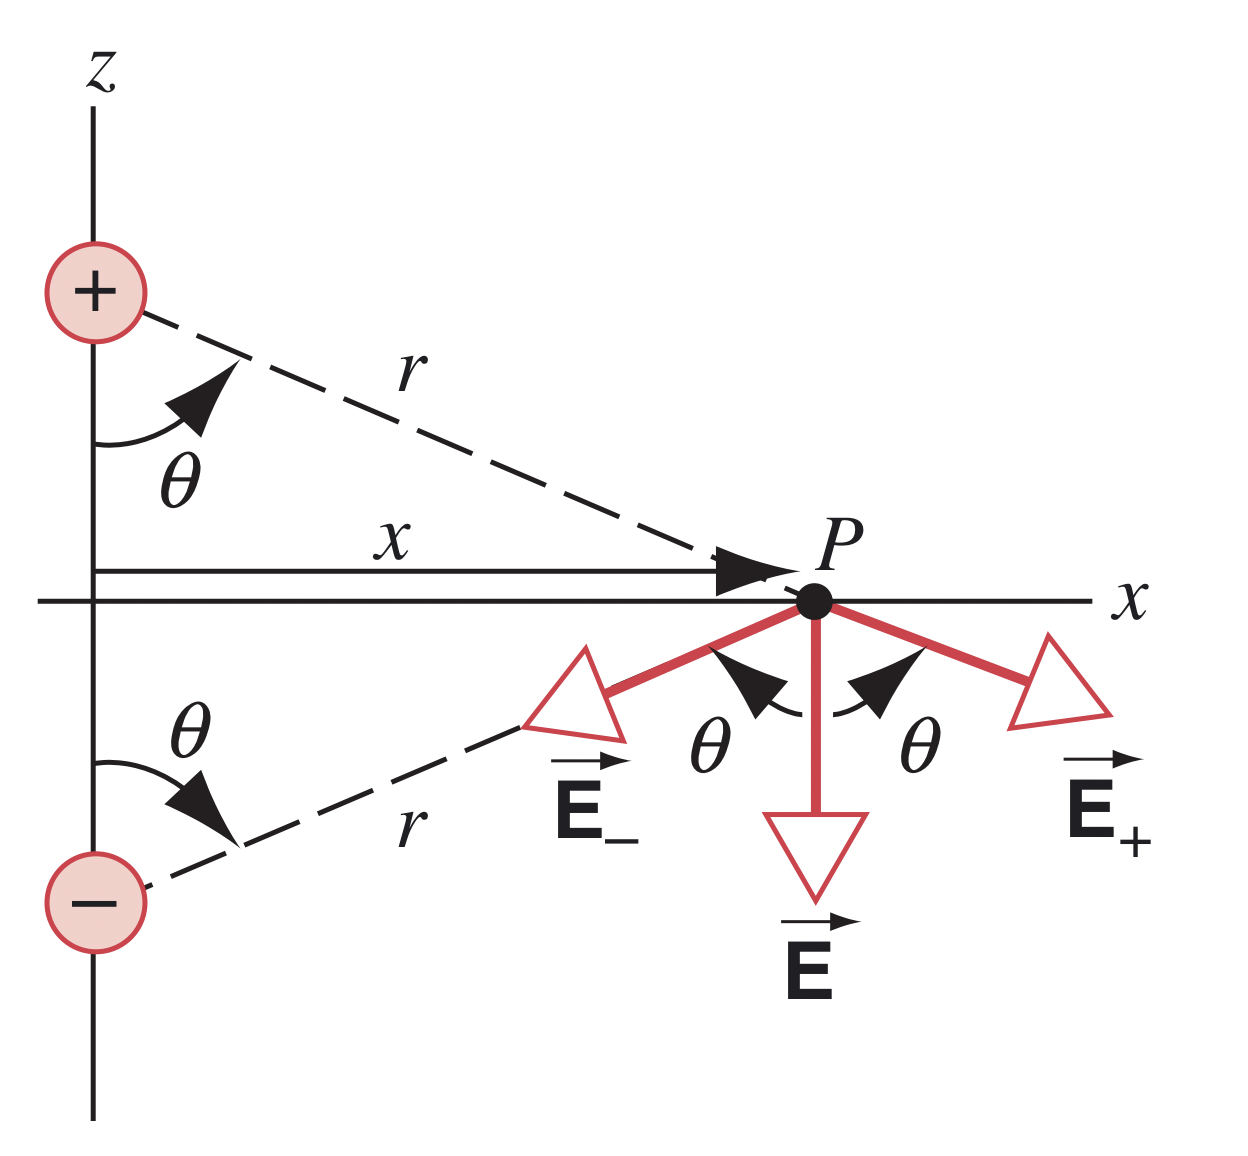
\includegraphics[width=0.8\textwidth]{dipole}
  \caption{The field at any is the vector sum of the charges.}
\end{marginfigure}
%
such that the work done by the field is
\begin{equation}
  W = - \int_{\theta_0}^\theta \tau \; d \theta = pE(\Delta \cos \theta)
\end{equation}
Consequently, the potential energy is defined as
\begin{equation}
  U = -pE \cos \theta = - \b p \cdot \b E
\end{equation}

\section{Potentials}
\emph{Gauss' Law} states the electric \emph{flux} through a field is
\begin{equation}
  \Phi_E = \oiint \b E \cdot d \b A = \frac{q}{\varepsilon_0}
\end{equation}
%
\begin{marginfigure}
  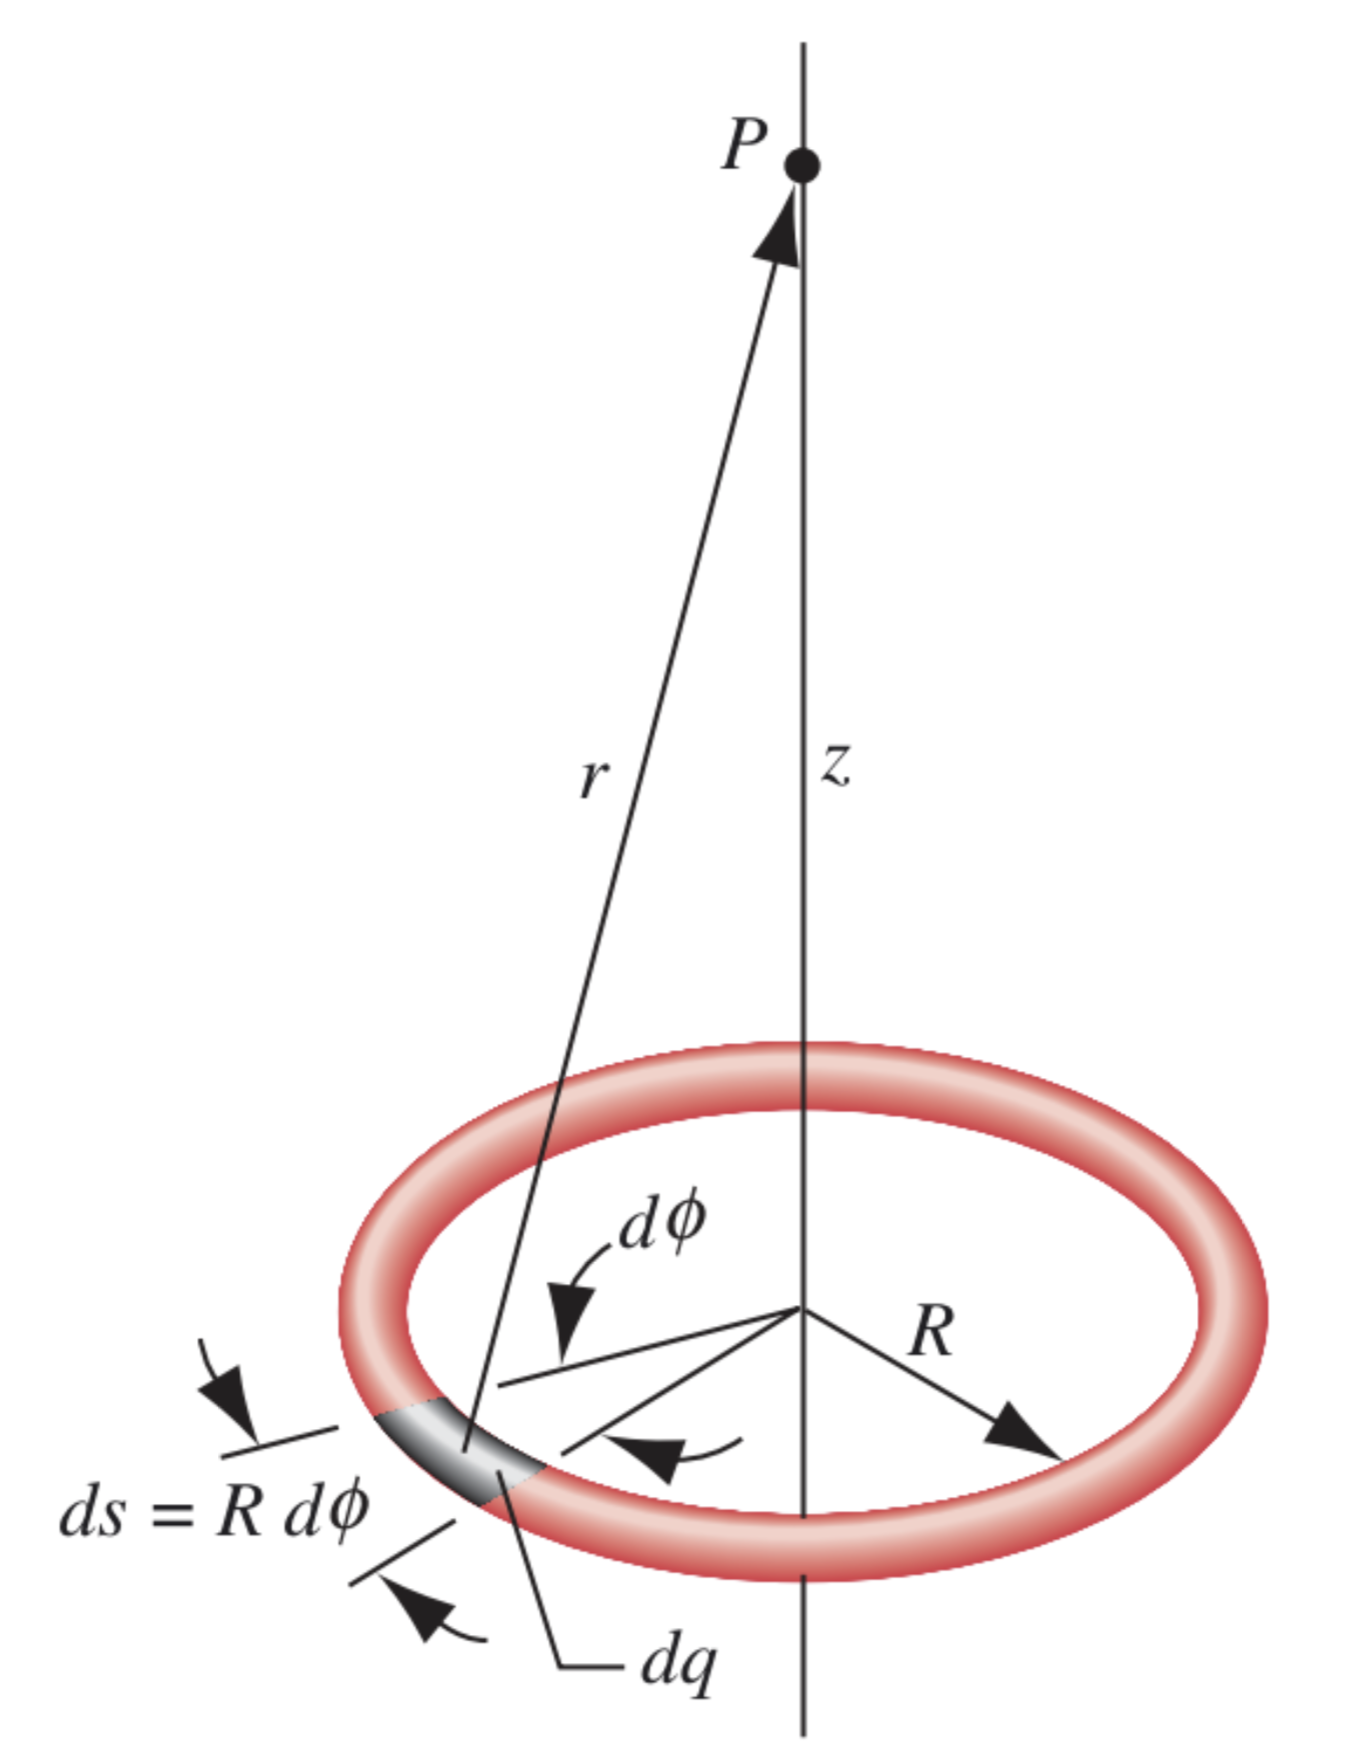
\includegraphics[scale=0.15]{potential}
  \caption{A uniformly charged ring with a potential $P$ and charge element $dq$.}
\end{marginfigure}
%
such that $\| \Phi \| = EA \cos \theta$ where $\theta$ is the angle between the field and field lines. The electric field outside a conductor is given by  \begin{equation}
  E = \frac{\sigma}{\varepsilon_0} \iff q = \iint \sigma \; dA
\end{equation}
The change in electric potential is defined as
\begin{equation}
  \Delta U = kq_1q_2 (\Delta r^{-1})
\end{equation}
For a system of charge, the \emph{potential energy} is
\begin{equation}
  U = k \sum_i \sum_{j\neq i} \frac{q_iq_j}{\r}
\end{equation}
Consequently, the change in \emph{electric potential} is
\begin{equation}
  \Delta V = \frac{\Delta U}{q_0} = - \frac{W}{q_0} = - \int \b E \cdot d \b s
\end{equation}
%
\begin{marginfigure}
  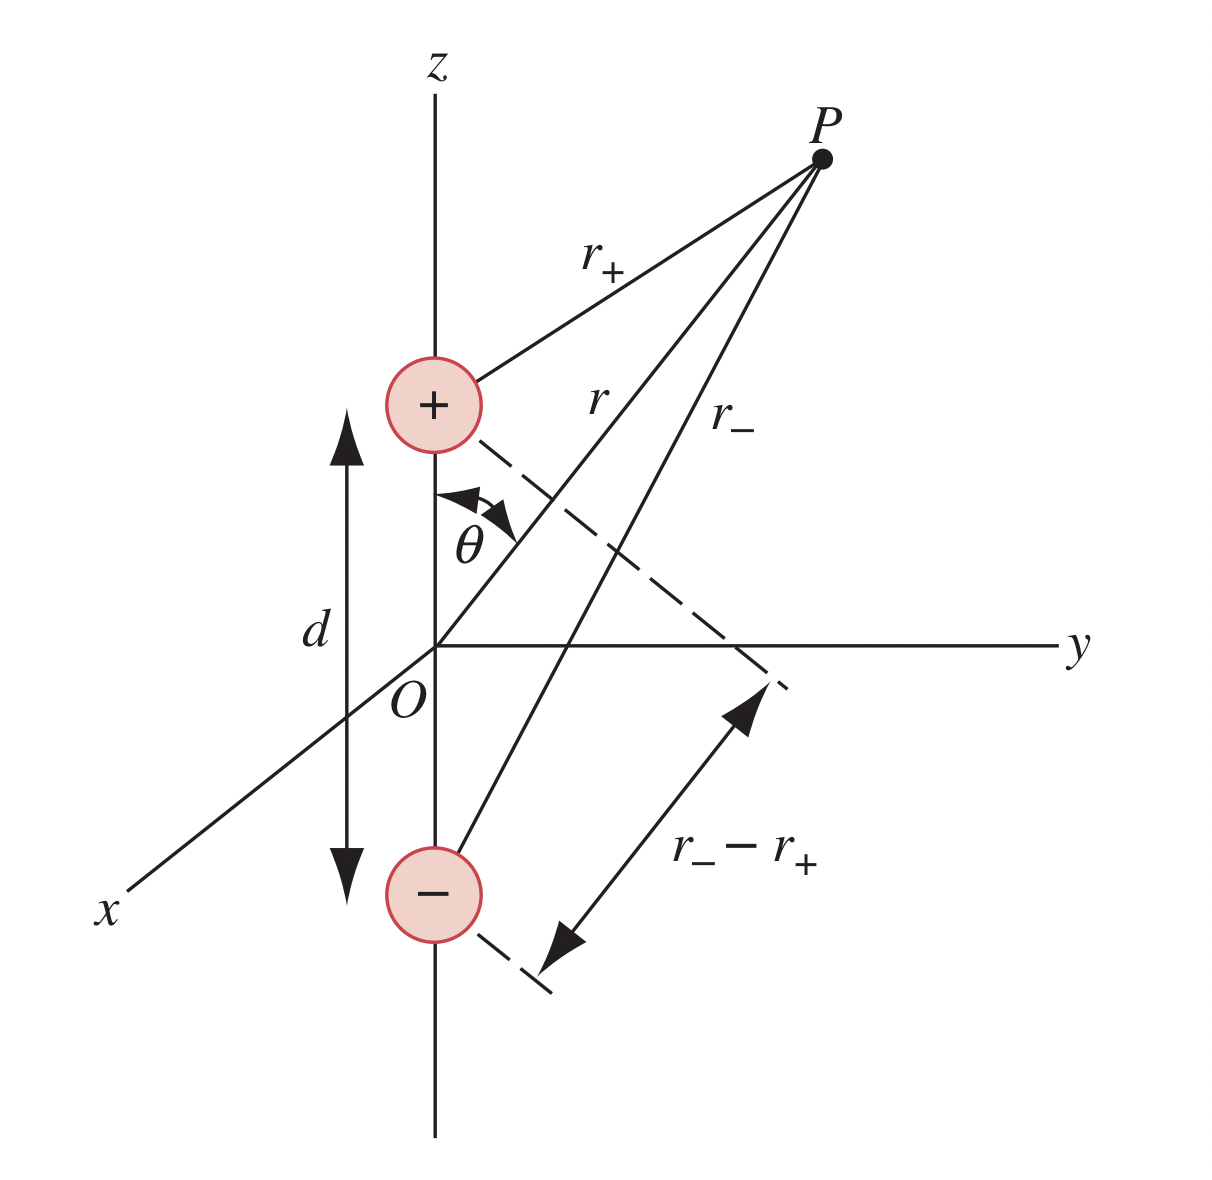
\includegraphics[width=1\textwidth]{dipole2}
  \caption{The geometry for calculating $V$ at $P$ for a dipole.}
\end{marginfigure}
%
The electric potential at a point is thus defined as
\begin{equation}
  V = k \iiint^b_a \frac{dq}{\r} = k \sum \frac{q_i}{\r} \sim k \frac{p \cos \theta}{\r^2}
\end{equation}
where the latter equivalence holds for dipoles. A surface on which the potential has the same value everywhere is \emph{equipotential} such that $\Delta V = W = 0$. The field lines must everywhere be perpendicular to the equipotential surfaces, which implies all conductors are equipotential.

\section{Examples}
\begin{fullwidth}
\begin{enumerate}
    \item Given $i = 2.5 \times 10^4$ C/s and $t = 20$ $\mu$s, calculate the charge $q$.
    \item There is a semicircular ring of charge with radius $r$ and charge $Q$. Find $E$ at the center of the circle $P$.
    \item Let there be a square of length $a$ with 4 charges on the corners. The charges clockwise are $+q, -q,$ $-2q, +2q$. Find $F$ on the $+2q$ charge.
    \item For a square with charges $Q, q, Q, q$ on the corners, if $F_Q = 0$, relate $Q$ and $q$.
    \item Two charges $Q$ are $d$ apart. A charge $-q$ and mass $m$ are midway between them that is slightly displaced and released. Prove $-q$ has a period $(\epsilon_0 m \pi^3 d^3 / qQ)^{1/2}$.
    \item Prove $\tau = \b p \times \b E$ and $\Delta U = - \b p \cdot \b E$.
    \item (a) Consider a line charge of length $L$ with $\lambda$. The rod is aligned along $z$ and the centre of the rod is the origin. Find $E$ at a point $P$ a distance $y$ from the rod along its perpendicular bisector (the positive y axis). Use the substitution $z = y \sinh t$ and $1+\sinh2t=\cosh2t$. (b) Assume that the line charge extends from $[-\infty, \infty]$ along the $z$-axis. Calculate $E$.
\end{enumerate}
\end{fullwidth}


%--------------------------------------------------------------------
% ELECTROSTATICS
%--------------------------------------------------------------------

\chapter{Electrodynamics}

\section{Current}

\textsc{The electric} current is defined as
\begin{equation}
  i = \frac{dq}{dt} = \int \b j \cdot d \b A
\end{equation} where $j$ is the current density and is opposite the motion of electrons. The net charge passing through is therefore
\begin{equation}
  q = \int i \, dt
\end{equation}
The current density is defined as
\begin{equation}
  \b j = q/At = - en \b v = \sigma \b E
\end{equation}
\begin{marginfigure}
  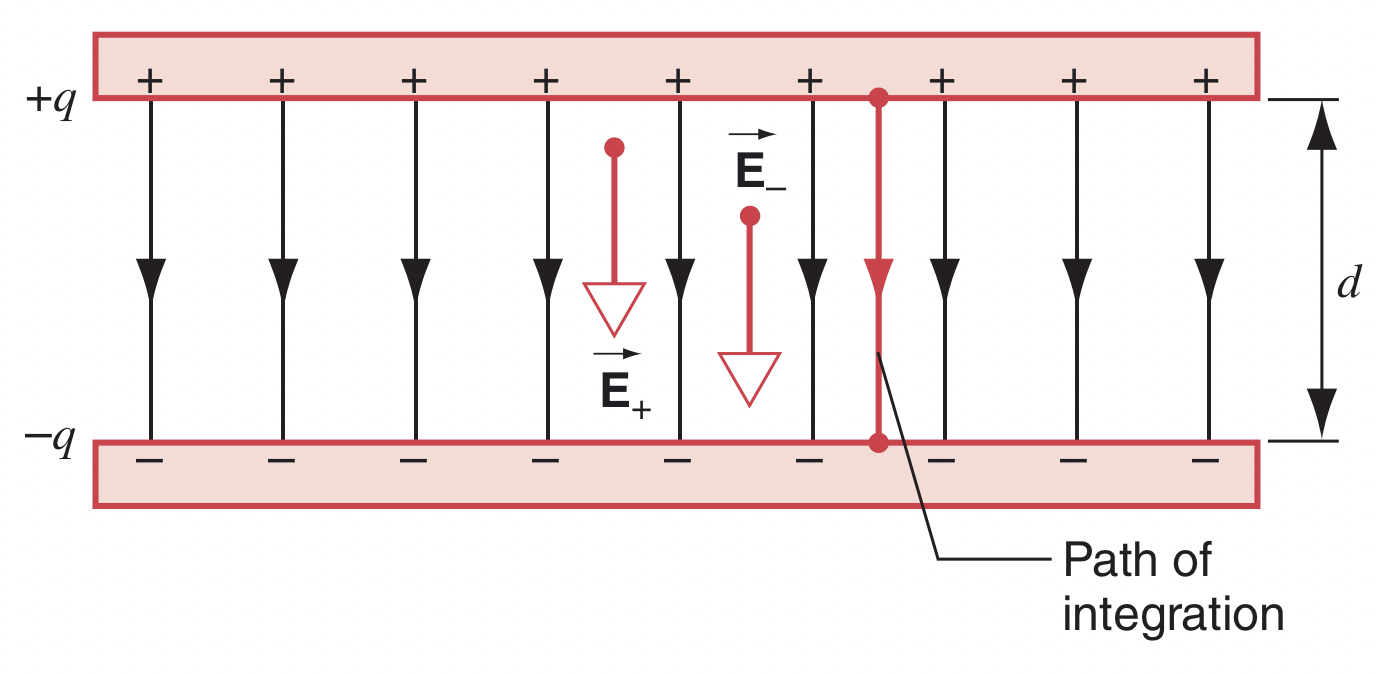
\includegraphics[width=1\textwidth]{ppc}
  \caption{A parallel-plate capacitor.}
\end{marginfigure}
where $n$ is the electron density and $\sigma = q/A$ is the conductivity. Furthermore, the net charge passing through the surface $q = enAL$. The resistance of the material is thus $R = L/\sigma A = \Delta V / i$.

\section{Capacitance}
\emph{Capacitance} is defined as
\begin{equation}
  C = \frac{q}{\Delta V} = \frac{\varepsilon_0 A}{d}
\end{equation}
In a PPC, SC, and CC, the potential is derived via
\begin{equation}
  \Delta V_{ppc} = \frac{qd}{\epsilon A} \qquad \Delta V_{sc} =kq \left(\frac{1}{a} - \frac{1}{b} \right) \qquad \Delta V_{ss} = \frac{q \ln (b-a)}{2 \pi \epsilon L}
\end{equation}
In a parallel combination of capacitors,
\begin{equation}
  q = \sum q  = C_{eq} \Delta V \iff  C_{eq} = \sum C
\end{equation}
and in a series combination,
\begin{equation}
  \Delta V = \sum \Delta V = q/C_{eq} \iff C_{eq}^{-1} = \sum C^{-1}
\end{equation}
As well, the potential energy in a capacitor is
\begin{equation}
  dU = \Delta V \, dq \iff U = \int_0^q dU = \frac{q^2}{2C}
\end{equation}
with $q = C \Delta V$. Specifically, the energy $U$ is stored in $E$ in the region. Furthermore, the \emph{energy density} $u$ is defined as \begin{equation}
  u = \frac{U}{Ad} = \textstyle\frac{1}{2} \varepsilon_0 E^2
\end{equation}
by Eqns 18 \& 22. Using \emph{voltage division}, the voltage of any impedance $Z$ including capacitance may be found via $q_0 = \sum q$ by \begin{equation}
  V = \frac{Z_1}{Z_{eq}} V_0
\end{equation}
For a \emph{dielectric capacitor}, the charge is defined as
\begin{equation}
  q' = q (1 - 1/\kappa) \iff E = E_0/\kappa
\end{equation}

\section{DC Circuits}
%
\begin{marginfigure}
  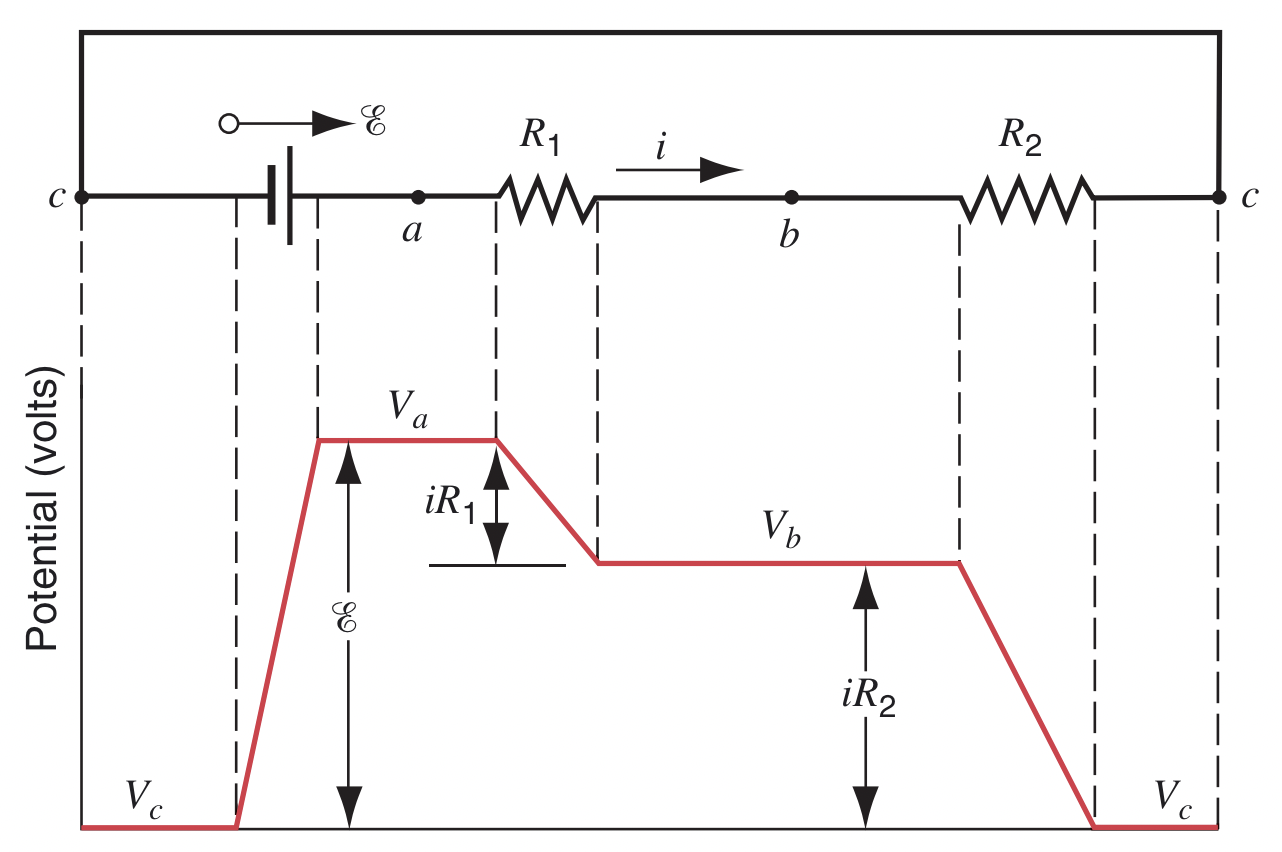
\includegraphics[width=1\textwidth]{dc}
  \caption{A simple circuit and its potential difference change.}
\end{marginfigure}
%
The \emph{emf} of a voltage source is defined as \begin{equation}
    \mathcal E = dW/dq = iR
\end{equation}
The electric potential $v$ decreases across a voltage source in a circuit.

\bigskip
\begin{center}
    \fbox{\textit{For more information, view the Electric Circuits textbook supplement.}}
\end{center}
\bigskip

The emf is related to the electric field by \begin{equation}
    \mathcal E = \oint \b E \cdot d \b s
\end{equation}
where $\b E = \b F/q = \rho j$.

%--------------------------------------------------------------------
% MAGNETOSTATICS
%--------------------------------------------------------------------

\chapter{Magnetic Forces}

\section{Magnetic Field}
The magnetic force is defined as \begin{equation}
    \b F = q \b v \times \b B \qquad \| \b F \| = |q| v B \sin \phi
\end{equation}
where $B$ is the field and $v$ the velocity. The combined electric and magnetic fields yield the Lorentz force,
%
\begin{marginfigure}
  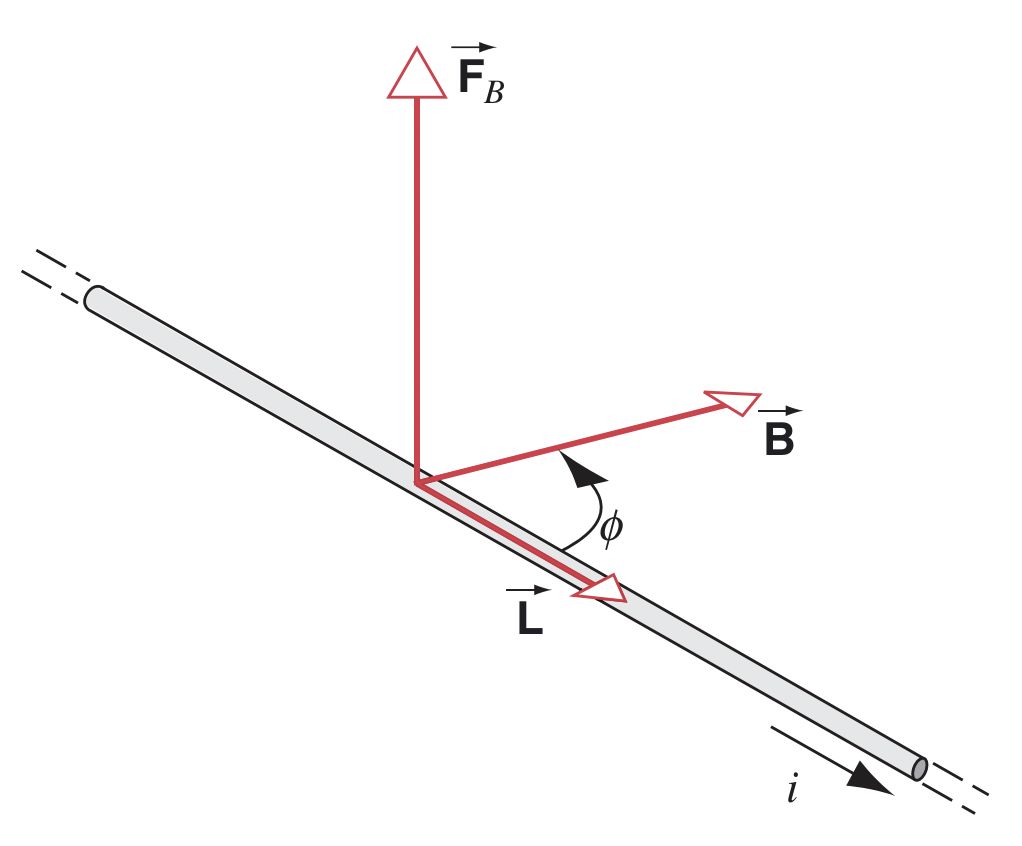
\includegraphics[width=0.8\textwidth]{wire}
  \caption{$\b F$ acting on a wire $\b L$ making an angle $\phi$ with $\b B$.}
\end{marginfigure}
%
\begin{equation}
    \b F = q \b E + q \b v \times \b B
\end{equation}
For a velocity selector, then $v = E/B$, and for a particle in a circular path, then: \begin{equation}
    |q|v B = mv^2/r \qquad \omega = v/r = |q|B/m
\end{equation}
where $\omega = 2 \pi f = r'$ is the angular velocity, and the kinetic energy is $K = 0.5 mv^2$.

\bigskip
The Hall effect states for a strip of conductor, the electric field is \begin{equation}
    \b E_H = - \b v_d \times \b B
\end{equation}
which gives $n = iB/et \Delta V_H$. For a straight wire, then \begin{equation}
    \b F = i \b L \times \b B \sim iLB \sin \phi
\end{equation}
For a uniform non-straight wire, $dF = iB \, ds$. The total torque on such wire being rotated is given by
%
\begin{marginfigure}
  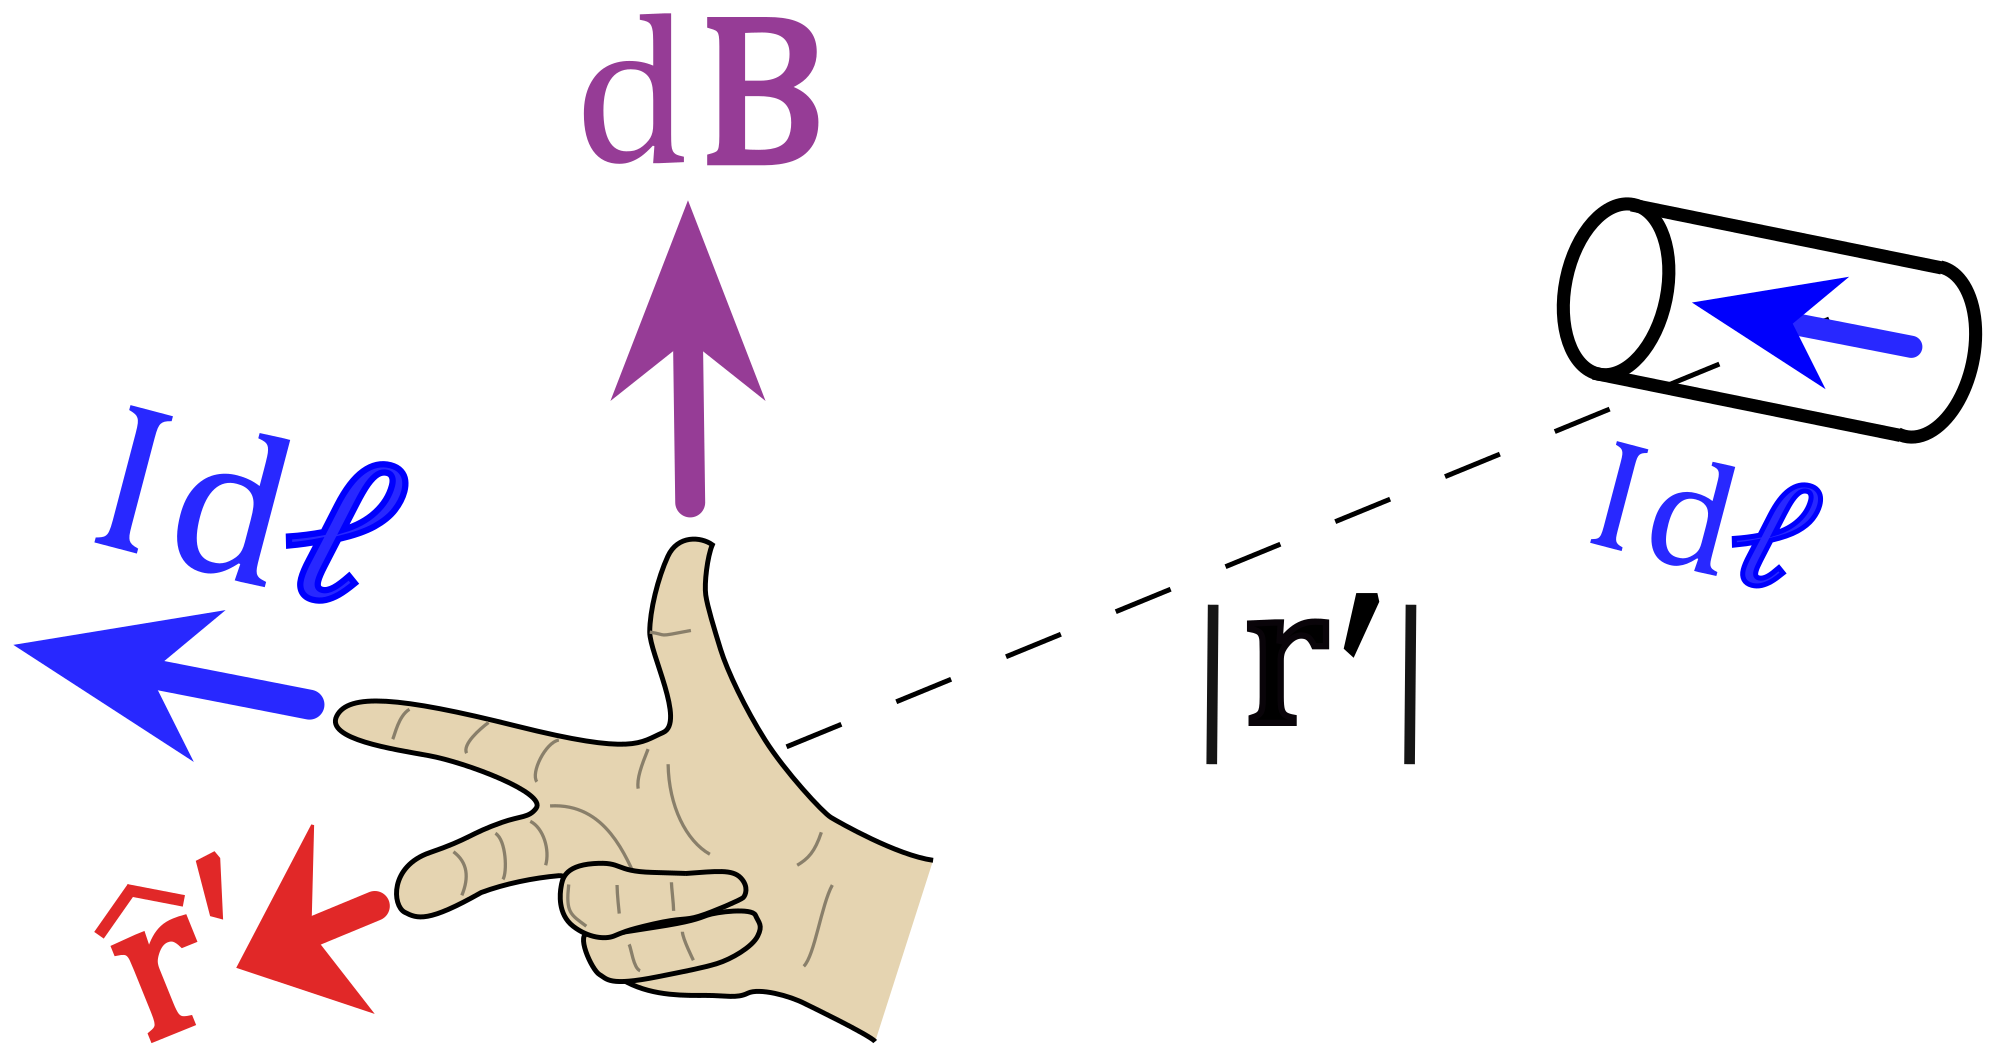
\includegraphics[width=0.6\textwidth]{rhr}
  \caption{The right hand rule for magnetic field lines.}
\end{marginfigure}
%
\begin{equation}
    \tau = NIA \b n \times \b B
\end{equation}

\section{Alternate Definition}
The magnetic field may also be expressed as \begin{equation}
    \b B = K \frac{|q| v \sin \phi}{r^2} = K \int_C \frac{i \, d \b s \times \mathbf{\hat{r}}}{r^2}
\end{equation}
where $i \, d \b s = dq \, v$, known as the Biot-Savart law. For two parallel wires in a magnetic field, the force of wire 1 on 2 is \begin{equation}
    F_{21} = i_2 LB_1 = \frac{KL i_1i_2}{d}
\end{equation}
Note antiparallel currents repel. Ampere's law generalizes the magnetic field to state \begin{equation}
    \oiint \b B \cdot d \b s = \mu_0 i
\end{equation}

\end{document}
